\documentclass[fleqn, a4paper, 12pt]{article}
\usepackage{amsmath, amssymb, amsthm}
%\usepackage{gensymb}
\usepackage{commath}
\usepackage{xcolor}
\usepackage{cancel}
\usepackage{siunitx}
\usepackage{tikz, pgfplots}
\usetikzlibrary{calc, hobby, patterns}
\usepackage{graphicx}
\usepackage{hyperref}
\usepackage{datetime}
\usepackage{ulem}
\usepackage{xfrac}
\usepackage{enumerate}
\setcounter{secnumdepth}{4}
\newcommand\numberthis{\addtocounter{equation}{1}\tag{\theequation}}

\newcommand{\AxisRotator}[1][rotate=0]{%
	\tikz [x=0.25cm,y=0.60cm,line width=.2ex,-stealth,#1] \draw (0,0) arc (-150:150:1 and 1);%
}

\theoremstyle{definition}
\newtheorem{example}{Example}
\newtheorem{definition}{Definition}

\theoremstyle{theorem}
\newtheorem{theorem}{Theorem}

\newenvironment{solution}
{\begin{proof}[Solution]\let\qed\relax}
	{\end{proof}}

\newcommand{\curl}{\mathrm{curl\,}}

%\renewcommand{\int_{min}^{max}}{\int\displaylimits_{min}^{max}}

%opening
\title{Lecture 12}
\author{Aakash Jog}
\date{\formatdate{4}{12}{2014}}

\begin{document}

\maketitle
%\setlength{\mathindent}{0pt}

\tableofcontents

\newpage
\section{Impulse and Momentum}

\begin{example}
	Assuming a plastic collision, what is the maximum compression of the string?\\
	\begin{tikzpicture}
		%definition of origin
		\coordinate (O) at (0,0,0); 
		
		%definition of minimum and maximum values for axes
		\def\xMIN{-1};
		\def\yMIN{-1};
		\def\xMAX{2};
		\def\yMAX{2};
		
		%axes
%		\draw [<->, lightgray] (\xMIN,0,0) -- (\xMAX,0,0) node [right] {$x$}; 
%		\draw [<->, lightgray] (0,\yMIN,0) -- (0,\yMAX,0) node [above] {$y$};
		
		%definition of variables
		\def\L{2};
		\def\H{2};
		
		%
		\draw (-2,0) -- (2,0);
		
		\draw [decorate, decoration={coil, segment length=5pt, aspect=0.7}] (O) -- node [midway, right] {$k$} ++(90:\L) coordinate (spring top) ;
		
		\draw [ultra thick] (spring top)+ (-1,0) -- ++(1,0) node [right] {$m_2$};
		
		\draw (spring top) ++(0,\H) circle [radius=3pt] coordinate (initial m1) node [right] {$m_1$};
		
		\draw [|<->|] (initial m1)++ (2,0) -- ++(-90:\H) node [midway, fill=white] {$H$};
		
		\draw [|<->|] (spring top)++ (2,0) -- ++(-90:\L) node [midway, fill=white] {$L$};
		
		\draw [dashed, red] (spring top) -- ++(180:4) node [left] {$U = 0$};
	\end{tikzpicture}
\end{example}

\begin{solution}
	Applying COME before the collision,
	\begin{align*}
		m_1 g H &= \dfrac{1}{2} m_1 v_1^2\\
		\therefore v_1 &= \sqrt{2 g H}
	\end{align*}
	The spring is already compressed due to $m_2$. Therefore
	\begin{align*}
		k x_i &= m_2 g\\
		\therefore x_i &= \dfrac{m_2 g}{k}
	\end{align*}
	Therefore, the natural length of the spring is
	\begin{align*}
		x_i + L &= \dfrac{m_2 g}{k} + L
	\end{align*}
	Applying COLM during the collision,
	\begin{align*}
		m_1 v_1 &= (m_1 + m_2) u_{12}\\
		\therefore u_{12} &= \dfrac{m_1}{m_1 + m_2} v_1
	\end{align*}
	Applying COME after the collision,
	\begin{align*}
		\dfrac{1}{2} (m_1 + m_2) u_{12}^2 + 0 + \dfrac{1}{2} k x_i^2 &= 0 + (m_1 + m_2) g (-x_{\text{max}}) + \dfrac{1}{2} k (x_i + x_{\text{max}})^2
	\end{align*}
\end{solution}

\begin{example}
	Find $x_2$.\\
	\begin{tikzpicture}
		%definition of origin
		\coordinate (O) at (0,0,0); 
		
		%definition of minimum and maximum values for axes
		\def\xMIN{-1};
		\def\yMIN{-1};
		\def\xMAX{2};
		\def\yMAX{2};
		
		%axes
		%		\draw [<->, lightgray] (\xMIN,0,0) -- (\xMAX,0,0) node [right] {$x$}; 
		%		\draw [<->, lightgray] (0,\yMIN,0) -- (0,\yMAX,0) node [above] {$y$};
		
		%definition of variables		
		\def\v0{2};
		\def\alpha{60};
		
		\def\X{8};
		\def\H{3};
		
		\def\x{3};
		\def\y0{2};
		
		\coordinate (apex) at ({\X/2}, \H);
		
		%
		\draw (O) -- (0:10);
		\fill (O) circle [radius = 2pt] node [below left] {$m_1 + m_2$};
		
		\draw [->] (O) -- ++(\alpha:\v0) node [midway, left] {$v_0$};
		\draw [dashed](O) to [out=\alpha, in= 180] ({\X/2}, \H) to [out = 0, in={180 - \alpha}] (0:\X);
		
		\fill (apex) circle [radius = 2pt];
		
		\draw [->, blue] (apex) -- ++(0:2) node [right] {$u_1$};
		\draw [->, red] (apex) -- ++(180:1.5) node [left] {$u_2$};
		
	\end{tikzpicture}
\end{example}

\begin{solution}
	Applying COLM,
	\begin{align*}
		(m_1 + m_2) v_0 \cos \alpha &= m_1 u_1 + m_2 u_2
	\end{align*}
	\begin{align*}
		v_y &= v_0 \sin \alpha - g t_1\\
		\therefore 0 &= v_0 \sin \alpha - g t_1\\
		\therefore t_1 &= \dfrac{v_0 \sin \alpha}{g}
	\end{align*}
	\begin{align*}
		u_1 t &= x_1\\
		\therefore u_1 \dfrac{v_0 \sin \alpha}{g} &= x_1\\
		\therefore u_1 &= \dfrac{x_1 g}{v_0 \sin \alpha}
	\end{align*}
\end{solution}

\section{Variable Mass Systems}

\begin{example}
	For a body, given $\dod{M}{t} = \rho A v$, find $v_t$.
\end{example}

\begin{solution}
	Let the velocity and mass of the body at time $t$ be $v$ and $m$ respectively. Therefore, applying COLM,
	\begin{align*}
		m_0 v_0 &= m v\\
		\therefore m &= \dfrac{m_0 v_0}{v}\\
		\therefore \dod{M}{t} &= - \dfrac{m_0 v_0}{v^2} \cdot \dod{v}{t}\\
		\therefore \rho A v &= - \dfrac{m_0 v_0}{v^2} \cdot \dod{v}{t}\\
		\therefore \int\limits_{v_0}^{v} \dfrac{\dif v}{v^3} &= \int\limits_{0}^{t} \dfrac{\rho A}{m_0 v_0} \dif t\\
		\therefore \dfrac{1}{2 v^2} - \dfrac{1}{2 v_0^2} &= \dfrac{\rho A}{m_0 v_0} t 
	\end{align*}
\end{solution}

\begin{example}
	Given $m_0$ is the initial mass of the rocket, $\dod{m}{t} = -k$, and $u$ is the velocity of the gas emitted from the rocket relative to the rocket, find the rocket's velocity as a function of time.
\end{example}

\begin{solution}
	\begin{align*}
		\dif p &= p_{t + \dif t} - p_{t}
	\end{align*}
	At $t$,\\
	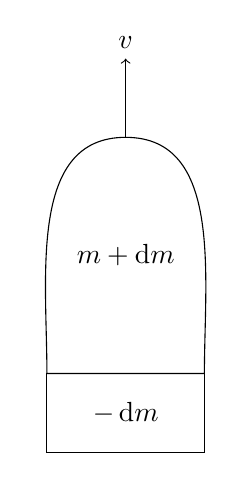
\begin{tikzpicture}
		\draw (-1,0) to [out=90, in=180] (0,3) to [out=0, in=90](1,0) -- cycle;
			\node at (0,1.5) {$m + \dif m$};
		\draw (-1,0) rectangle node {$-\dif m$} (1,-1);
		
		\draw [->] (0,3) -- ++(90:1) node [above] {$v$};
	\end{tikzpicture}
	\begin{align*}
		P_t &= m v
	\end{align*}
	At $t + \dif t$,\\
	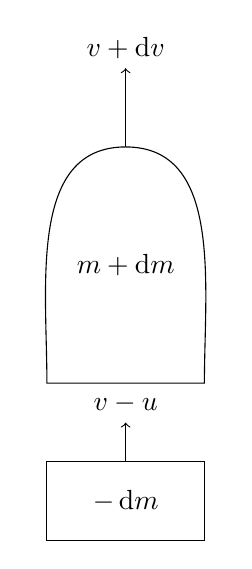
\begin{tikzpicture}
	\draw (-1,0) to [out=90, in=180] (0,3) to [out=0, in=90](1,0) -- cycle;
		\node at (0,1.5) {$m + \dif m$};
	\draw [yshift = -1cm] (-1,0) rectangle node {$-\dif m$} (1,-1);
	
	\draw [->] (0,3) -- ++(90:1) node [above] {$v + \dif v$};
	\draw [->] (0,-1) -- ++(90:0.5) node [above] {$v - u$};
	\end{tikzpicture}
	\begin{align*}
	p_{t + \dif t} &= (m + \dif f) (v + \dif v) + (- \dif m) (v - u)
	\end{align*}
	\begin{align*}
		\dif p &= p_{t + \dif t} - P_t\\
		&= m \dif v + \cancel{\dif m v} +\dif m \dif v - \cancel{\dif m v} + \dif m u\\
		\therefore \dod{p}{t} &= M \dod{v}{t} + \cancelto{0}{\dod{m}{t} \dif v} + \dod{m}{t} u\\
		&= M \dod{v}{t} + \dod{m}{t} u
	\end{align*}
	\begin{align*}
		- m g &= \dod{p}{t}\\
		&= M \dod{v}{t} + \dod{m}{t} u\\
		&= m \dod{v}{t} - k u\\
		\therefore m \dod{v}{t} &= k u - m g
	\end{align*}
	Therefore the rocket accelerates upwards iff
	\begin{align*}
		k u - m g &> 0\\
		\iff k u &> m g
	\end{align*}
	Therefore, the condition for take-off is
	\begin{equation*}
		k u > m_0 g
	\end{equation*}
	\begin{align*}
		\dod{m}{t} &= -k\\
		\therefore m&= m_0 - k t
	\end{align*}
	\begin{align*}
		m \dod{v}{t} &= k u - m g\\
		\therefore (m_0 - k t) \dod{v}{t} &= k u - (m_0 - k t)g\\
		\therefore \int\limits_{0}^{v} \dif v &= \int\limits_{0}^{t} \left( \dfrac{k u}{m_0 - k t} - g \right) \dif t\\
		&= - u \ln (m_0 - k t) + u \ln m_0 - g t\\
		&= u \ln \left(\dfrac{m_0}{m_0 - k t}\right) - g t\\
		\therefore v(t) &= u \ln \left(\dfrac{m_0}{m_0 - k t}\right) - g t
	\end{align*}
\end{solution}

\begin{example}
	\hspace{1cm}\\
	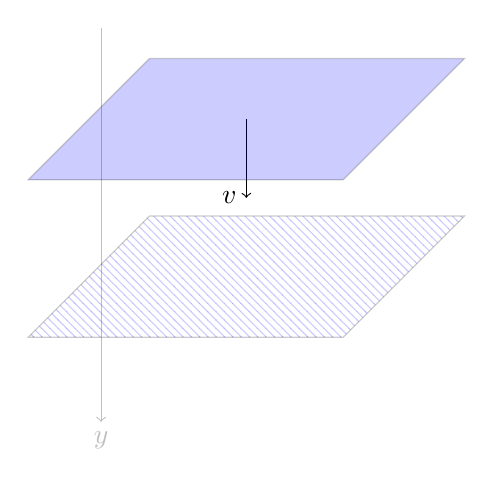
\begin{tikzpicture}
		%definition of origin
		\coordinate (O) at (0,0,0); 
		
		%definition of minimum and maximum values for axes
		\def\xMIN{-3};
		\def\yMIN{-3};
		\def\zMIN{-3};
		\def\xMAX{2};
		\def\yMAX{2};
		\def\zMAX{2};
		
		%axes
%				\draw [<->, lightgray] (\xMIN,0,0) -- (\xMAX,0,0) node [right] {$x$}; 
				\draw [->, lightgray] (0,\yMAX,0) -- (0,\yMIN,0) node [below] {$y$};
%				\draw [<->, lightgray] (0,0,\yMIN) -- (0,0,\zMAX) node [above] {$z$};
		%		
		
		\draw [->] (3,2,3) -- (3,1,3) node [left] {$v$};
		\filldraw [opacity = 0.2, fill = blue] (1,2,1) -- (5,2,1) -- (5,2,5) -- (1,2,5) -- cycle; 
		
		\filldraw [opacity = 0.2, pattern = north west lines, pattern color = blue] (1,0,1) -- (5,0,1) -- (5,0,5) -- (1,0,5) -- cycle; 
	\end{tikzpicture}
\end{example}

\begin{solution}
	\begin{align*}
		p_t &= m \cdot v + \rho A v \dif t \cdot 0\\
		p_{t + \dif t} &= (m + \rho A v \dif t) (v + \dif v)\\
		\therefore \dif p &= m \dif v + \rho A v^2 \dif t + \rho A v \dif v \dif t\\
		\therefore \dod{p}{t} &= m \dod{v}{t} + \rho A v^2 + \rho A v \dif v
	\end{align*}
\end{solution}

\end{document}